Single high-order element subdomains can be used in place of subdomains consisting of multiple low-order elements.
This approach has been investigated for solid mechanics problems, such as in \cite{pavarino2010bddc}; although, this work incorporated additional primal degrees of freedom from average values across subdomain edges and faces.

\begin{table}[ht!]
\begin{center}
\begin{tabular}{l ccc ccc}
  \toprule
  $p$  &  \multicolumn{3}{c}{Lumped BDDC}  &  \multicolumn{3}{c}{Dirichlet BDDC}  \\
                      &  $\lambda_{\text{min}}$  &  $\lambda_{\text{max}}$  &  $\kappa$ & $\lambda_{\text{min}}$  &  $\lambda_{\text{max}}$ & $\kappa$  \\
  \toprule
  $p = 2$   &  1.000  &    2.800  &    2.800  &  1.000  &  2.042  &  2.042  \\
  $p = 4$   &  1.000  &   12.948  &   12.948  &  1.000  &  3.242  &  3.242  \\
  $p = 8$   &  1.000  &   59.563  &   59.563  &  1.000  &  5.197  &  5.197  \\
  $p = 16$  &  1.000  &  289.678  &  289.678  &  1.000  &  7.761  &  7.761  \\
  \bottomrule
\end{tabular}
\end{center}
\caption{Condition Numbers and Maximal Eigenvalues for Single High-Order Element Subdomains}
\label{table:high_order_element_bddc}
\end{table}

Table \ref{table:high_order_element_bddc} shows the maximal eigenvalues and condition numbers for the symbol of the BDDC preconditioned operator $\tilde{\mathbf{M}}^{-1}_i \left( \boldsymbol{\theta} \right) \tilde{{\color{burgundy}\mathbf{A}}} \left( \boldsymbol{\theta} \right)$ for the two-dimensional Poisson problem on single high-order element subdomains with varying polynomial orders.

The improved condition number, and therefore convergence, of the Dirichlet BDDC compared to the lumped BDDC is more significant for high-order elements.
With single high-order element subdomains, the Fast Diagonalization Method approximate inverse subdomain solver can be used for both the subdomain subassembled inverse and subdomain interior inverse, which eliminates the advantage in reduced setup costs for lumped BDDC.

\begin{figure}[!ht]
  \centering
  \subfloat[Lumped BDDC]{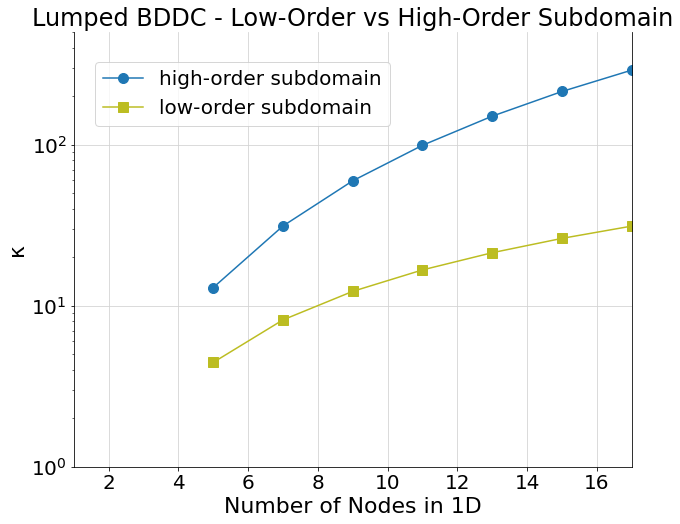
\includegraphics[width=0.48\textwidth]{../img/lowVsHighLumped}\label{fig:lumped_bddc_comparison}}
  \hfill
  \subfloat[Dirichlet BDDC]{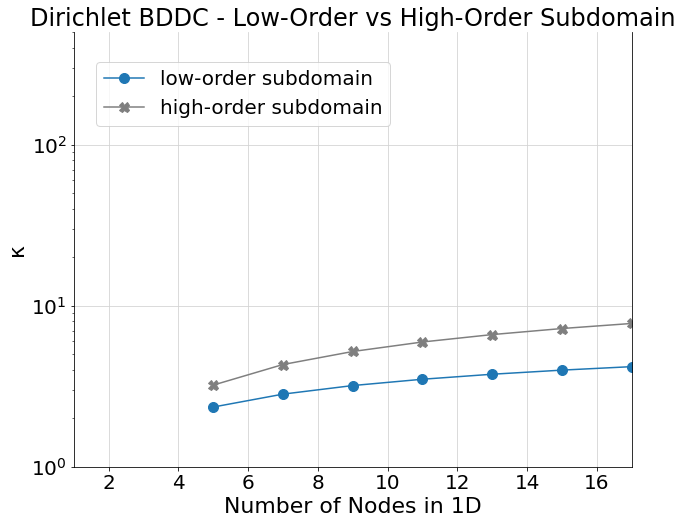
\includegraphics[width=0.48\textwidth]{../img/lowVsHighDirichlet}\label{fig:dirichlet_bddc_comparison}}
  \caption{Low-Order and High-Order Subdomain Condition Number Comparison}
\end{figure}

In Figure \ref{fig:lumped_bddc_comparison} we compare the growth of the condition number for the lumped BDDC preconditioned operator for a subdomain consisting of several linear elements and a subdomain consisting of a single high-order element for the two-dimensional Poisson problem.
The condition number grows much more rapidly for a high-order subdomain with an equivalent number of degrees of freedom.

In Figure \ref{fig:dirichlet_bddc_comparison} we compare the growth of the condition number for the Dirichlet BDDC preconditioned operator for a subdomain consisting of several linear elements and a subdomain consisting of a single high-order element for the two-dimensional Poisson problem.
In contrast with Figure \ref{fig:lumped_bddc_comparison}, we see that the condition number of the preconditioned operator on the high-order subdomain grows only slightly faster than the condition number of the low-order subdomain.

\begin{figure}[!ht]
  \centering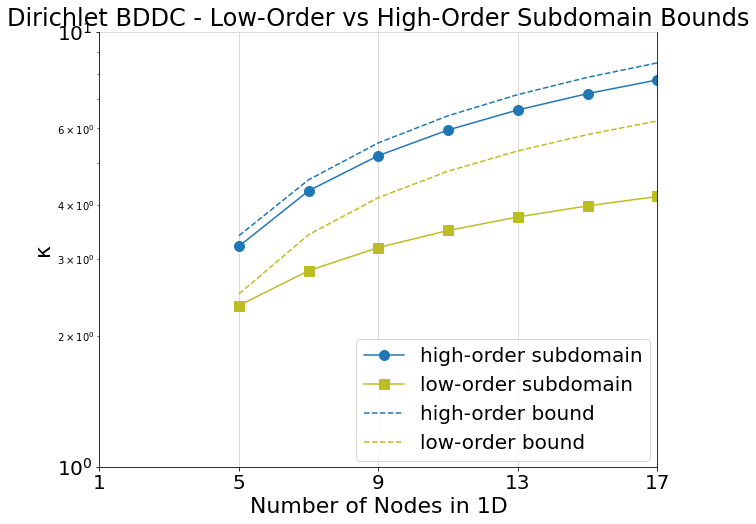
\includegraphics[width=0.52\textwidth]{../img/lowVsHighDirichletBounds}
  \caption{Low-Order and High-Order Subdomain Condition Number Bounds}
  \label{fig:dirichlet_bddc_bounds}
\end{figure}

The condition numbers of the Dirichlet BDDC preconditoner operator is bounded by
\begin{equation}
\kappa \leq \mathcal{C} \left( 1 + \log \left( p^2 \frac{H}{h} \right) \right)^2
\end{equation}
where $\mathcal{C} > 0$ is independent of the polynomial order $p$, the element size $h$, and the subdomain size $H$ \cite{klawonn2008spectral}.
In Figure \ref{fig:dirichlet_bddc_bounds}, we can see that our LFA-predicted condition numbers closely agree with this bound.

Klawonn, Pavarino, and Rheinbach investigated the performance of BDDC and FETI-DP preconditioners for the two-dimensional Poisson problem with discontinuous coefficients \cite{klawonn2008spectral} and provided some experimentally derived maximal eigenvalues and condition numbers for the two-dimensional Poisson problem.

\begin{table}[ht!]
\begin{center}
\begin{tabular}{l ccc ccc}
  \toprule
  $p$  &  \multicolumn{3}{c}{LFA}  &  \multicolumn{3}{c}{Experimental Results}  \\
                      &  $\lambda_{\text{min}}$  &  $\lambda_{\text{max}}$  &  $\kappa$ & $\lambda_{\text{min}}$  &  $\lambda_{\text{max}}$ & $\kappa$  \\
  \toprule
  $p = 2$   &  1.000  &   2.042  &   2.042  &  1.001  &   1.66  &   1.66  \\
  $p = 3$   &  1.000  &   2.614  &   2.614  &  1.000  &   2.38  &   2.38  \\
  $p = 4$   &  1.000  &   3.241  &   3.241  &  1.001  &   3.03  &   3.03  \\
  $p = 8$   &  1.000  &   5.195  &   5.194  &  1.001  &   5.01  &   5.00  \\
  $p = 16$  &  1.000  &   7.756  &   7.756  &  1.001  &   7.62  &   7.61  \\
  $p = 32$  &  1.000  &  10.961  &  10.961  &  1.002  &  10.86  &  10.84  \\
  \bottomrule
\end{tabular}
\end{center}
\caption{Condition Numbers and Maximal Eigenvalues for Dirichlet BDDC with Single Element High-Order Subdomains}
\label{table:high_order_bddc_experiments_1}
\end{table}

\begin{table}[ht!]
\begin{center}
\begin{tabular}{l ccc ccc}
  \toprule
  $p$  &  \multicolumn{3}{c}{LFA}  &  \multicolumn{3}{c}{Experimental Results}  \\
                      &  $\lambda_{\text{min}}$  &  $\lambda_{\text{max}}$  &  $\kappa$ & $\lambda_{\text{min}}$  &  $\lambda_{\text{max}}$ & $\kappa$  \\
  \toprule
  $p = 2$   &  1.000  &   2.700  &   2.700  &  1.001  &   2.33  &   2.33  \\
  $p = 3$   &  1.000  &   3.568  &   3.568  &  1.001  &   3.21  &   3.21  \\
  $p = 4$   &  1.000  &   4.305  &   4.305  &  1.002  &   4.00  &   3.99  \\
  $p = 8$   &  1.000  &   6.511  &   6.511  &  1.003  &   6.26  &   6.24  \\
  $p = 16$  &  1.000  &   9.354  &   9.354  &  1.002  &   9.16  &   9.14  \\
  $p = 32$  &  1.000  &  12.856  &  12.856  &  1.002  &  12.69  &  12.66  \\
  \bottomrule
\end{tabular}
\end{center}
\caption{Condition Numbers and Maximal Eigenvalues for Dirichlet BDDC 4 Element High-Order Subdomains}
\label{table:high_order_bddc_experiments_2}
\end{table}

In Table \ref{table:high_order_bddc_experiments_1} we see the LFA-predicted maximal eigenvalues and condition numbers for the scalar Poisson problem in two dimensions with constant coefficients compared to numerical results on a domain with 576 subdomains consisting of a single high-order finite element.
The LFA-predicted condition numbers generally agree with the experimental results, typically providing a mildly pessimistic prediction when compared to the experimental results.

In Table \ref{table:high_order_bddc_experiments_1} we see the LFA-predicted maximal eigenvalues and condition numbers for the scalar Poisson problem in two dimensions with constant coefficients compared to numerical results on a domain with 576 subdomains consisting of four high-order finite elements.